\section{Introduction} \label{sec:introduction}

Problem solving is a meanwhile well established field in cognitive psychology. Generally problem solving can be described as the search within a problem space. \cite{Newell1972}. The literature suggests that different sub processes of problem solving need to be considered in order to understand the whole process. The relevant sub-processes are the perception of the task, understanding the problem, activating foreknowledge, manipulating the given information, dividing the problem into subgoals, developing a plan, detecting errors and finding and validating results. The sub-processes of problem solving can also be investigated separately. Problem solving can also be defined by the attempt to transition from a given initial state to a goal state. Furthermore it is necessary that there must be some kind of barrier that does not allow to achieving the goal state directly. \cite{muesseler2015allgemeine}

In previous research some common methods of investigating problem solving have been established. The main goal is to identify the cognitive and neuronal processes of problem solving. A popular method is eye tracking because it allows to identify which informations of a problem are being looked at and also gives information about action planning. \cite{underwood2005}  Furthermore, neuropsychological studies are used to investigate which brain areas are responsible for certain aspects of problem solving. \cite{Karnath2006} In general there already are several tasks which are being used to investigate problem solving in behavioral studies. One example is the nine dot problem. The problem is to connect all nine dots of a 3x3 matrix with four continuous straight lines and without taking the pen of the paper (see Figure \ref{fig:ninedots}).

\begin{figure}[h]
\centering
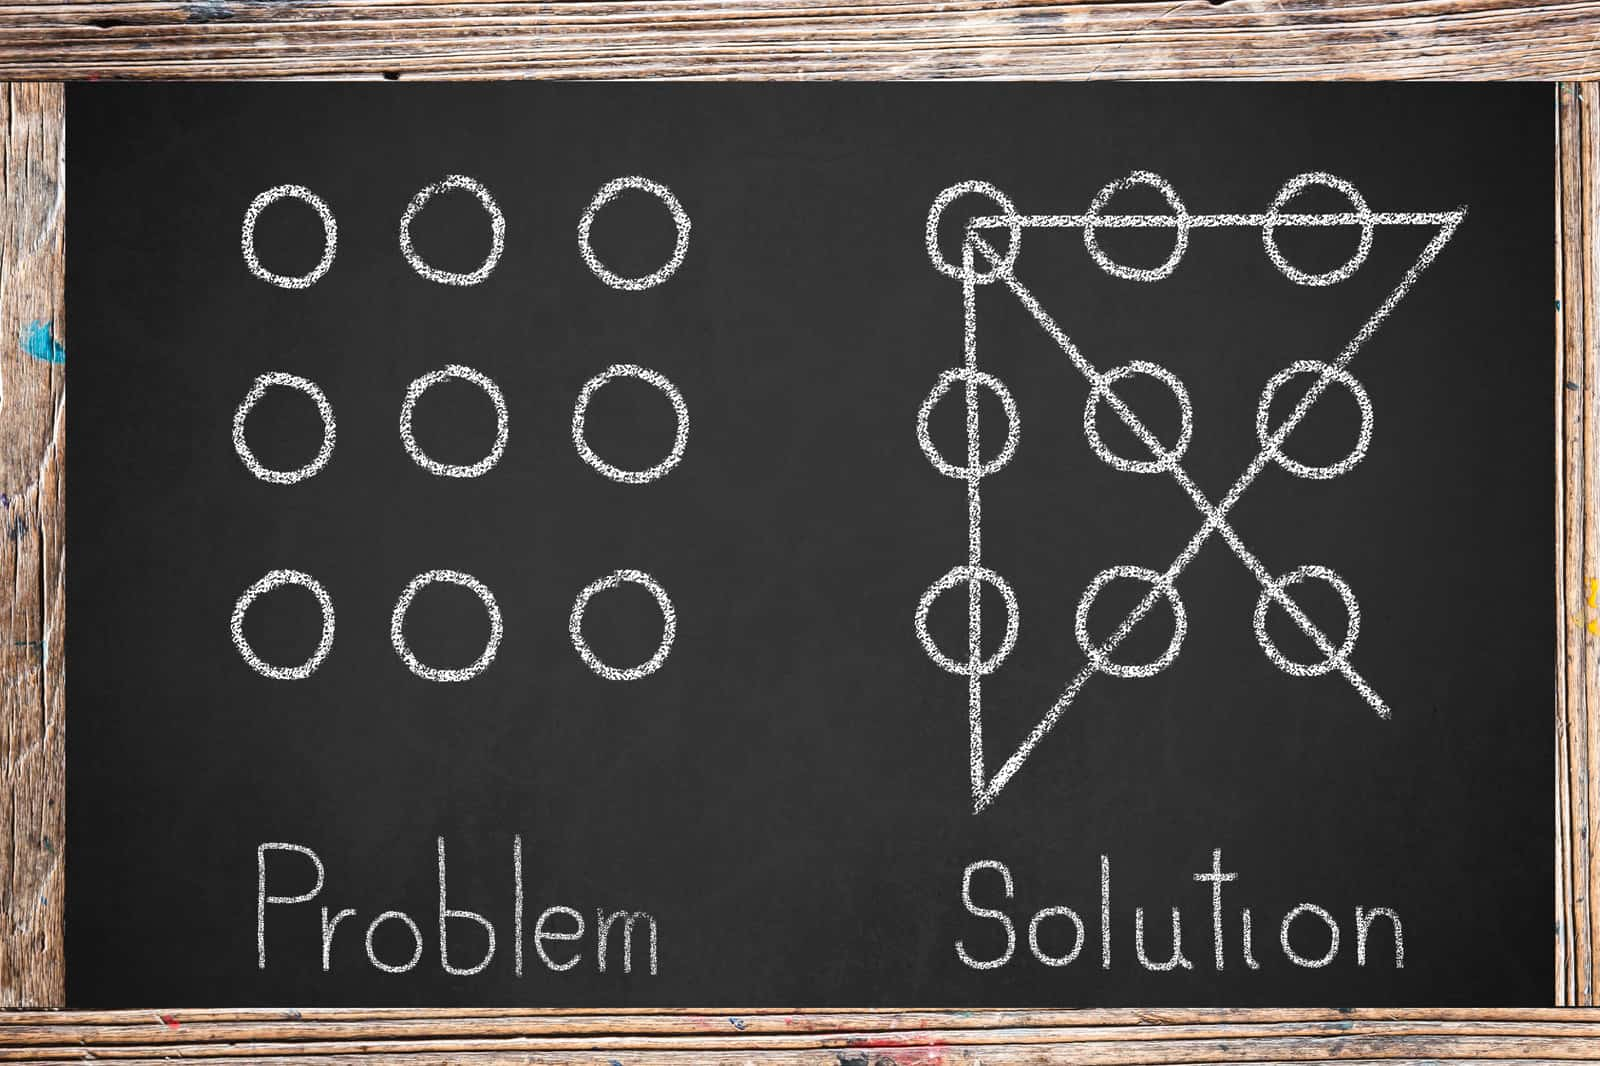
\includegraphics[width=0.5\textwidth]{ninedots}
\caption{Solution of the nine dot problem.}
\label{fig:ninedots}
\end{figure}

\newpage

In contrast to the more general approaches of problem solving described before, this work focuses on spatial problem solving and the question whether two people together perform better than a single person in a spatial problem solving task. 
Previous work in spatial problem solving has targeted fundamental processes of how individuals apply spatial learning, memory and planning. \cite{Waller2013} There also exist studies that investigate collaborative learning, but they do not focus on spatial problems. (e.g.  \cite{Dillenbourg1999} \cite{Hesse2015}) Therefore the main goal of this work is to investigate the combination of spatial and collaborative problem solving.  

Since it is quite difficult to investigate and measure performance in collaborative spatial problem solving tasks in the real world a new task in virtual reality has been designed for this study. This task has been designed in a way that allows to investigate and compare problem solving performance both in individuals and in groups of two. The main benefit of using virtual reality to investigate spatial problem solving is the fact that the technical equipment allows to easily record data of how participants interact with the virtual environment (e.g. controller movements and rotations). Furthermore in a virtual environment the task, the position of participants and the environmental aspects of the scene can be easily manipulated and controlled. Therefore, virtual reality appears to be a very promising method to investigate collaborative spatial problem solving. 

Only very few studies that compare to this approach of this study can be found. One example is the study by Heldal et al. from 2005. \cite{heldal2005}
The purpose of the study was to investigate differences in interfaces solving a virtual reality task similar to the Rubik's Cube like problem presented in this study. An example of the virtual scene that they used can be seen in Figure \ref{fig:heldal}. It has been shown that head mounted displays are one of the best interfaces to investigate spatial problem solving. Since then technology has rapidly developed and there are now much better interfaces and computer graphics available in order to create immersive virtual environments that allow interactions with different kinds of user input.

\begin{figure}[h]
\centering
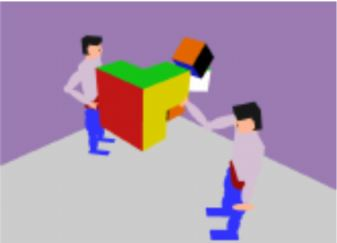
\includegraphics[width=0.5\textwidth]{heldal}
\caption{Virtual scene of the study by Heldal et al. from 2005. \cite{heldal2005}.}
\label{fig:heldal}
\end{figure}

 The main goal of this study was to design a task in a virtual environment that is suitable to investigate and quantify the performance in problem solving both in individuals and groups of two people and also compare both variations.